\newpage
\section*{Задание 1: Генерация изображения по текстовому запросу}
\subsection{Постановка задачи}
\noindent
Центральный объект: Умный светофор с камерами \\
Окружение / Фон: Перекрёсток мегаполиса под дождём \\
Стиль изображения: Кинематографичный кадр (как в кино) \\
Освещение: Ночное уличное, отражения на мокром асфальте \\
Обязательные детали: Объективы камер наблюдения, рамки выделения объектов (bounding boxes) вокруг машин \\
\subsection{Гипотеза и декомпозиция сцены}
\noindent
Перед генерацией сцена была разложена на ключевые компоненты для последующего включения в промпт:\\
Субъект: умный светофор, металлическая конструкция, встроенные камеры, объективы, датчики, светодиодные секции\\
Действие / Состояние: перекрёсток работает, машины проезжают, светофор показывает красный/зелёный\\
Окружение: перекрёсток мегаполиса, ночь, дождь, лужи на асфальте, небоскрёбы, мокрый асфальт\\
Освещение: ночное уличное, отражения огней в лужах, блики на мокрой дороге\\
Стиль:	кинематографичный кадр, глубокая резкость, кинематографический свет, атмосферный дождь\\
Обязательные детали:	камеры наблюдения на столбе, цветные рамки (bounding boxes) вокруг автомобилей, рамки выделения объектов\\
\subsection{Журнал генерации и отладки}
\textbf{Итерация 1 (наивный промпт)} \\
Промпт v1: «Умный светофор на перекрестке мегаполиса ночью под дождем, кинематографичный стиль»
% \newpage
\begin{figure}[H]
	\centering
	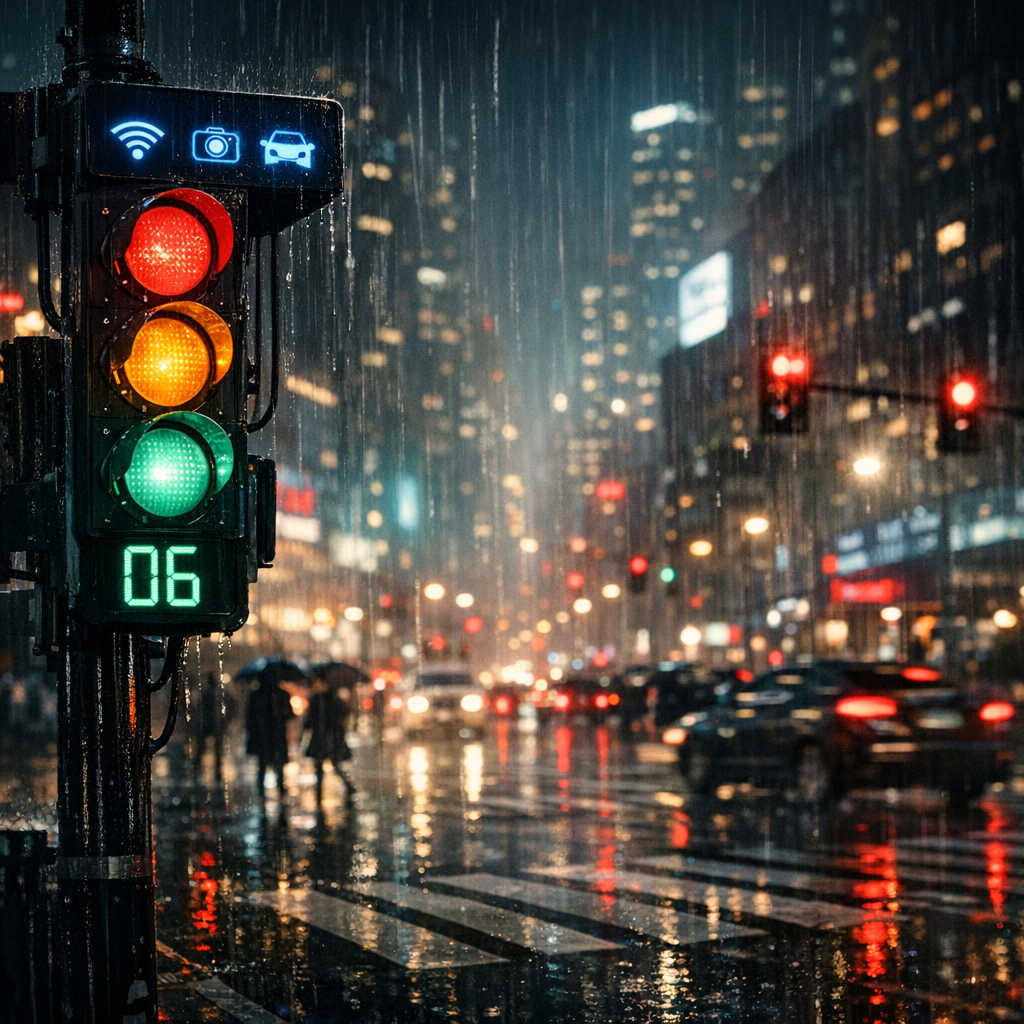
\includegraphics[width=17cm]{z1/1a.png}
	\caption{Итерация 1, модель (a)}
\end{figure}
\newpage
\begin{figure}[H]
	\centering
	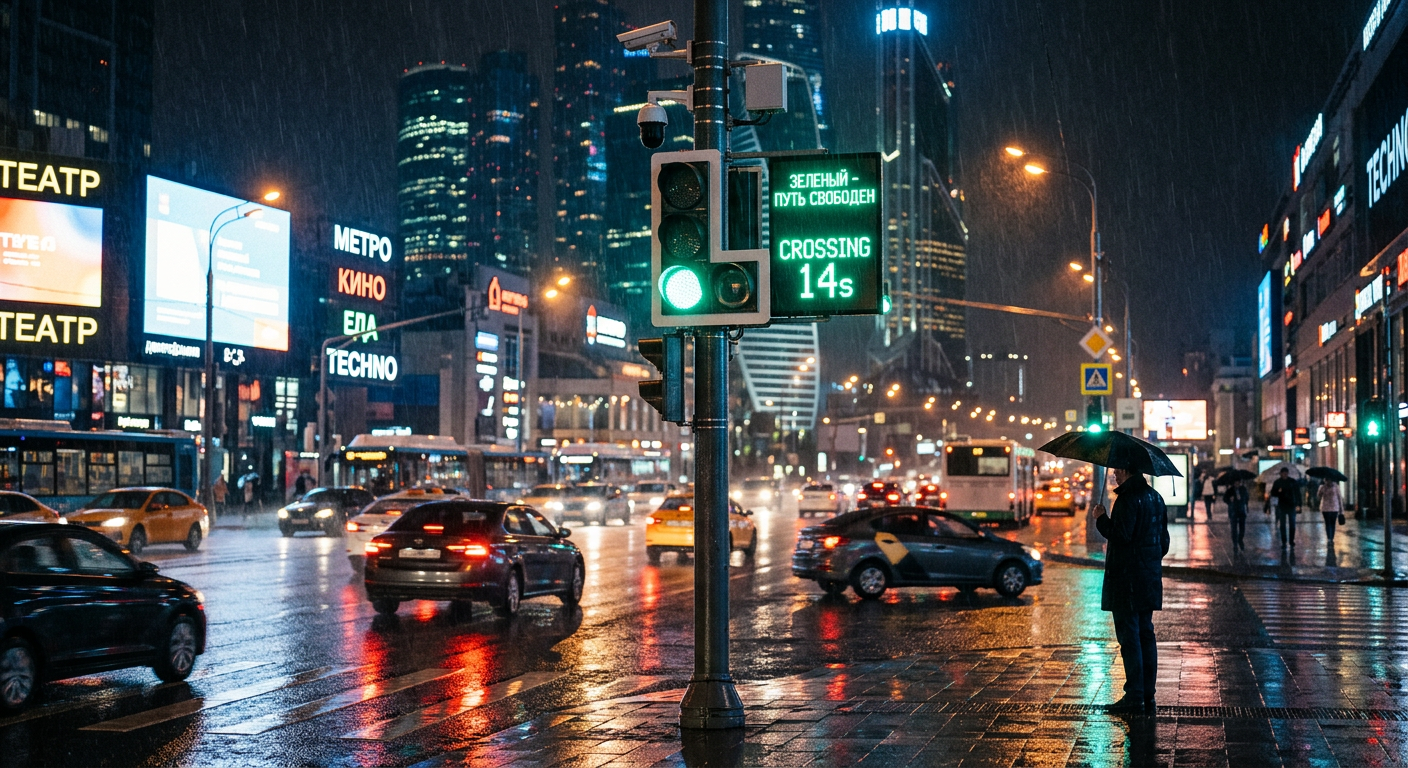
\includegraphics[width=17cm]{z1/1b.png}
	\caption{Итерация 1, модель (b)}
\end{figure}
\noindent \textbf{Анализ ошибок:}
Нет камер на светофоре (игнорирование важной детали).
Отсутствуют рамки вокруг машин. 
Стиль недостаточно «кинематографичный» (нет характерной цветокоррекции и глубины). \\
\noindent \textbf{Корректировка:}
Добавить явное упоминание «камеры наблюдения», «объективы», указать наличие цветных рамок вокруг машин, усилить стилистические маркеры («киношная цветокоррекция», «глубокий фокус»). \\
\newline
\textbf{Итерация 2 (уточнение деталей)} \\
Промпт v2: «Крупный план умного светофора с встроенными камерами наблюдения и объективами на перекрестке большого города ночью под дождем. На мокром асфальте яркие отражения фонарей и неона. Вокруг проезжающих автомобилей нарисованы цветные рамки выделения (bounding boxes) как в системах компьютерного зрения. Кинематографичный кадр, глубокая резкость, атмосферный дождь, киношная цветокоррекция.»
\begin{figure}[H]
	\centering
	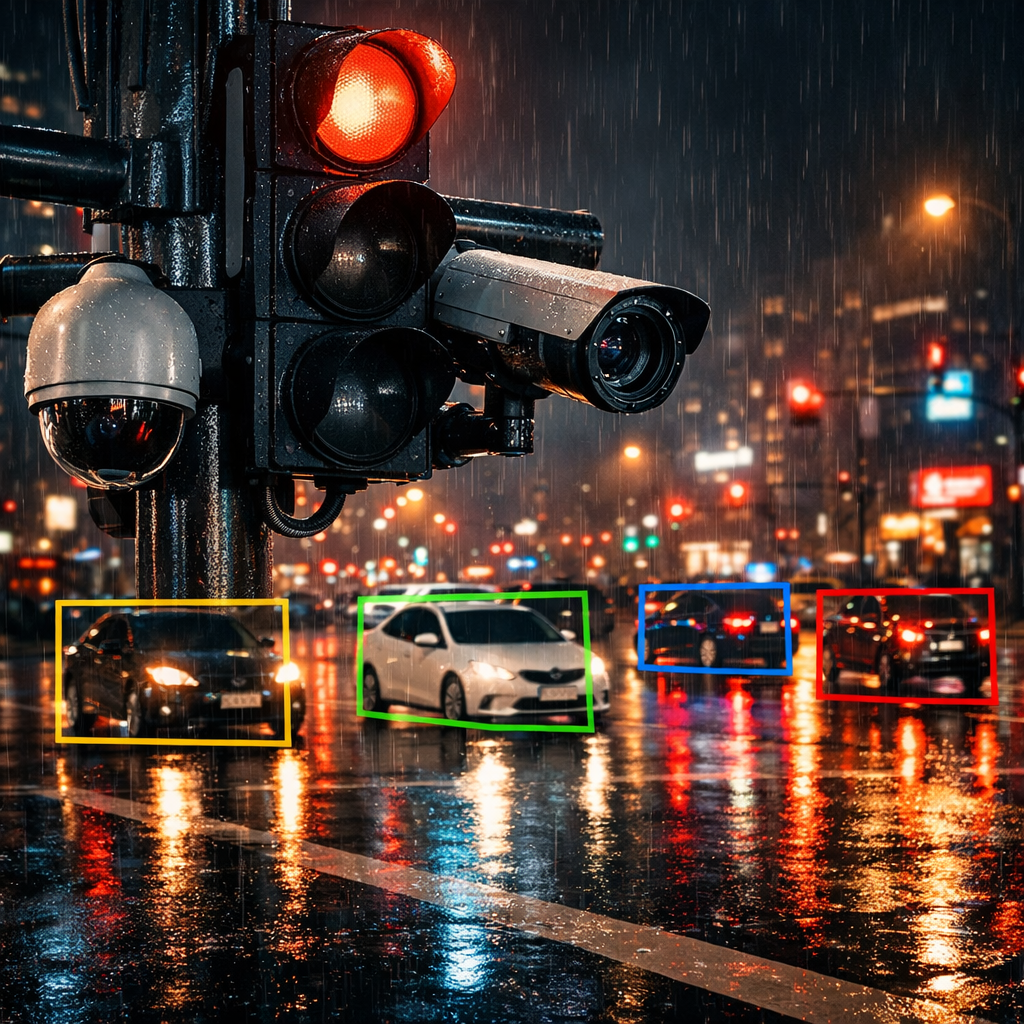
\includegraphics[width=17cm]{z1/2a.png}
	\caption{Итерация 2, модель (a)}
\end{figure}
У светофора неправильная перспектива, выглядит слишеом громоздко на изображении. Общая сцена мало похожа на перекрёсток.
\newpage
\begin{figure}[H]
	\centering
	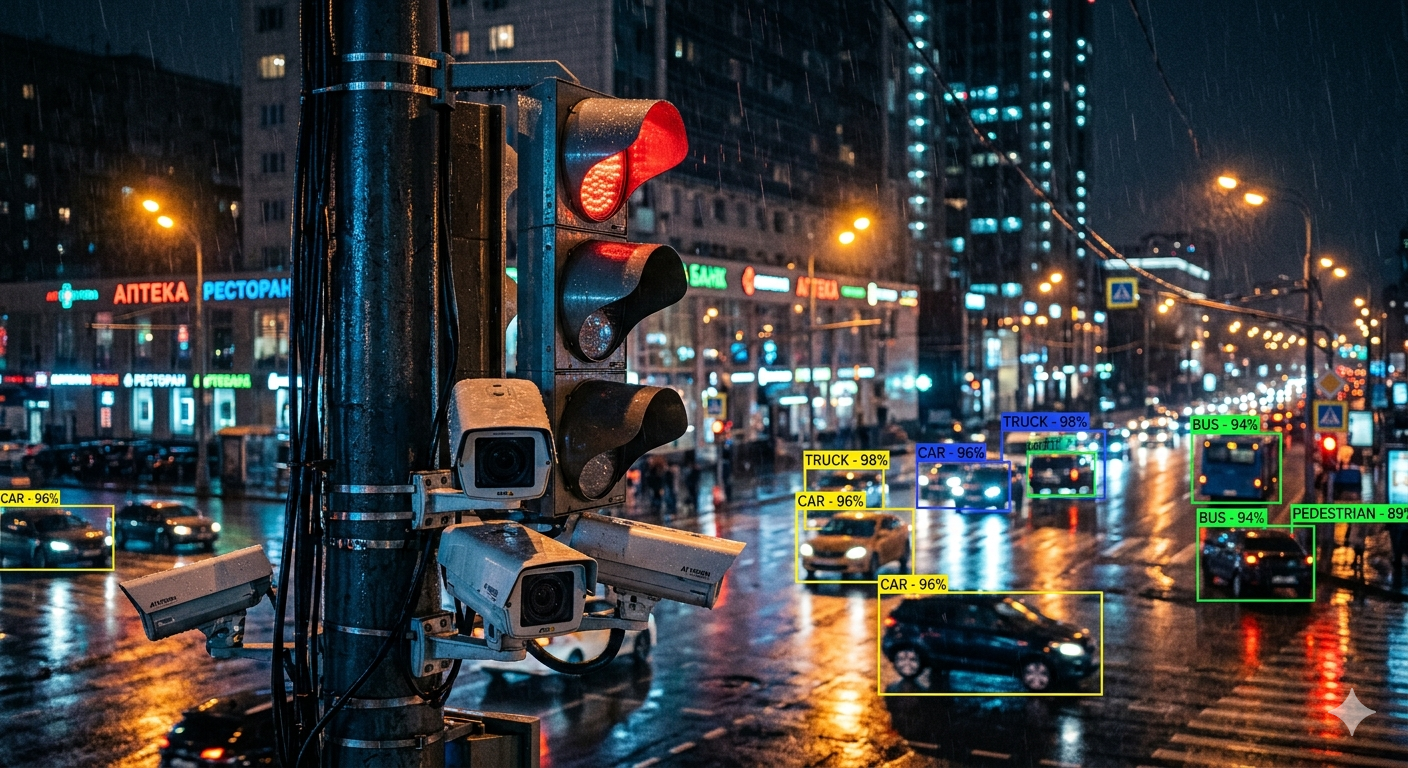
\includegraphics[width=17cm]{z1/2b.png}
	\caption{Итерация 2, модель (b)}
\end{figure}
Светофор корректно отображается крупным планом, рамки присутсвуют но не на всех автомобилях, некоторые рамки имеют неверную подпись. \\
\newline
\textbf{Анализ ошибок:}
Не все автомобили выделены рамкой, текст в рамке имеет случайный характер. \\
\textbf{Корректировка:}
Уточнить цвет рамки, указать текст раммки, а также указать конкретный транспорт.
\newline
\textbf{Итерация 3 (финальная)} \\
Промпт v3: «Крупный план умного светофора с встроенными камерами наблюдения и объективами на перекрестке большого города ночью под дождем. На мокром асфальте яркие отражения фонарей и неона. Вокруг каждого автомобиля нарисованы красные рамки выделения (bounding boxes) как в системах компьютерного зрения с текстом <<CAR \%>>, вокруг каждого автобуса жёлтые рамки с текстом <<BUS \%>> , вокруг людей и других объектов нет рамок. Кинематографичный кадр, глубокая резкость, атмосферный дождь, киношная цветокоррекция.»
\newpage
\begin{figure}[H]
	\centering
	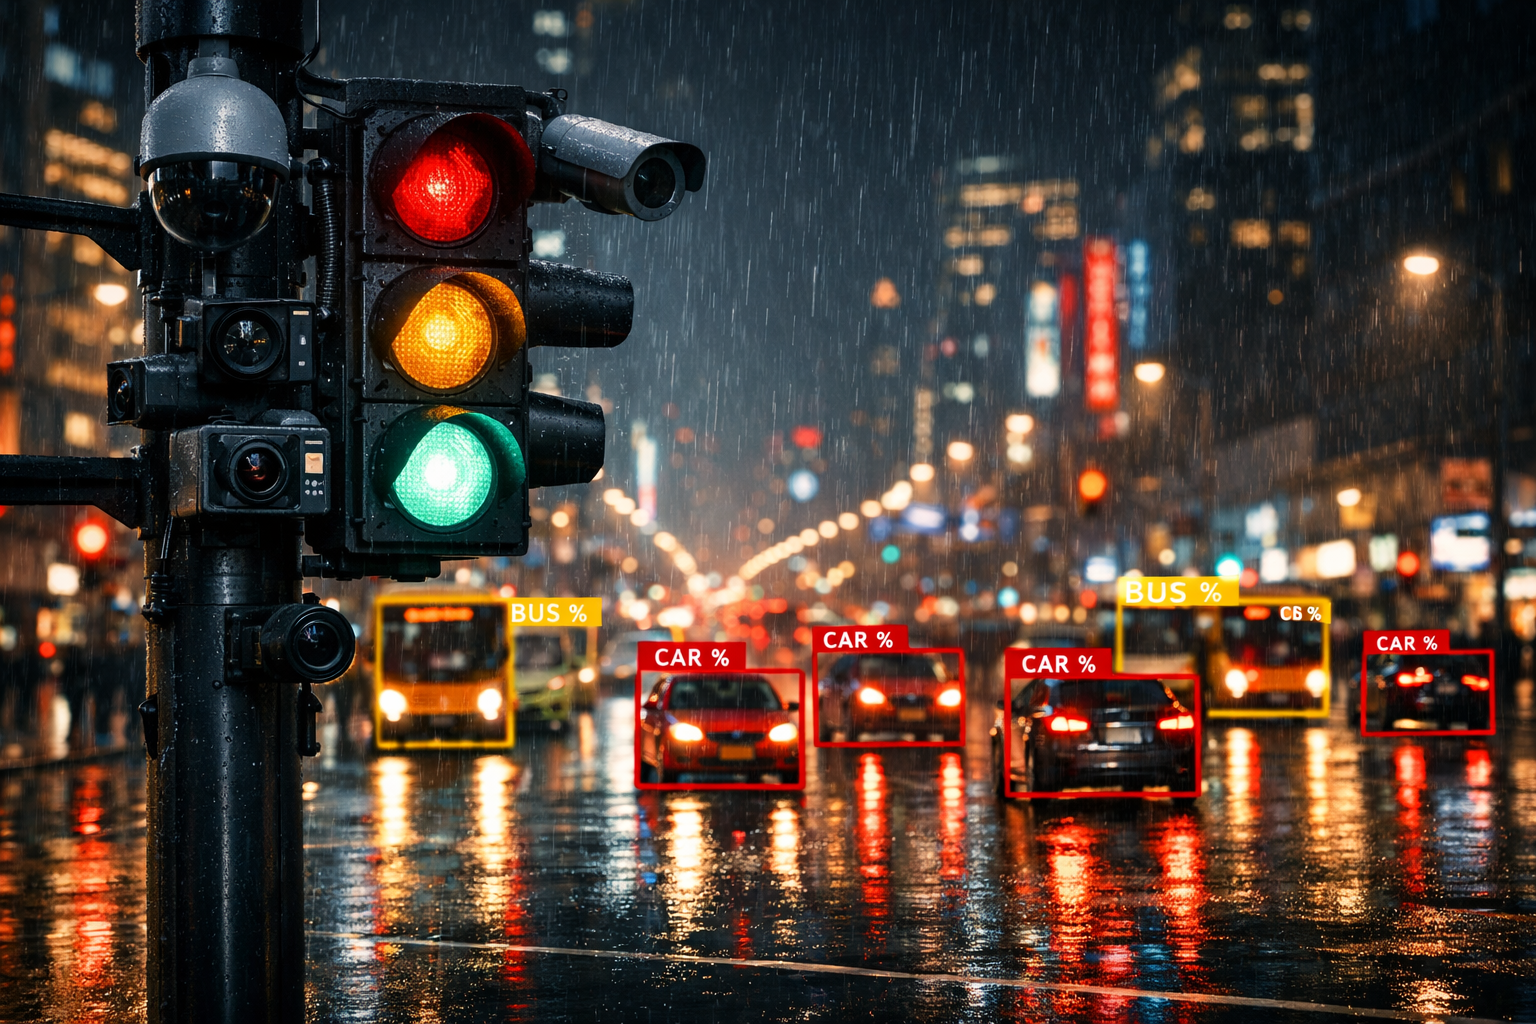
\includegraphics[width=17cm]{z1/3a.png}
	\caption{Итерация 3, модель (a)}
\end{figure}
В целом изображение соответствует заданию, но ощущается немного <<мыльным>>.
\newpage
\begin{figure}[H]
	\centering
	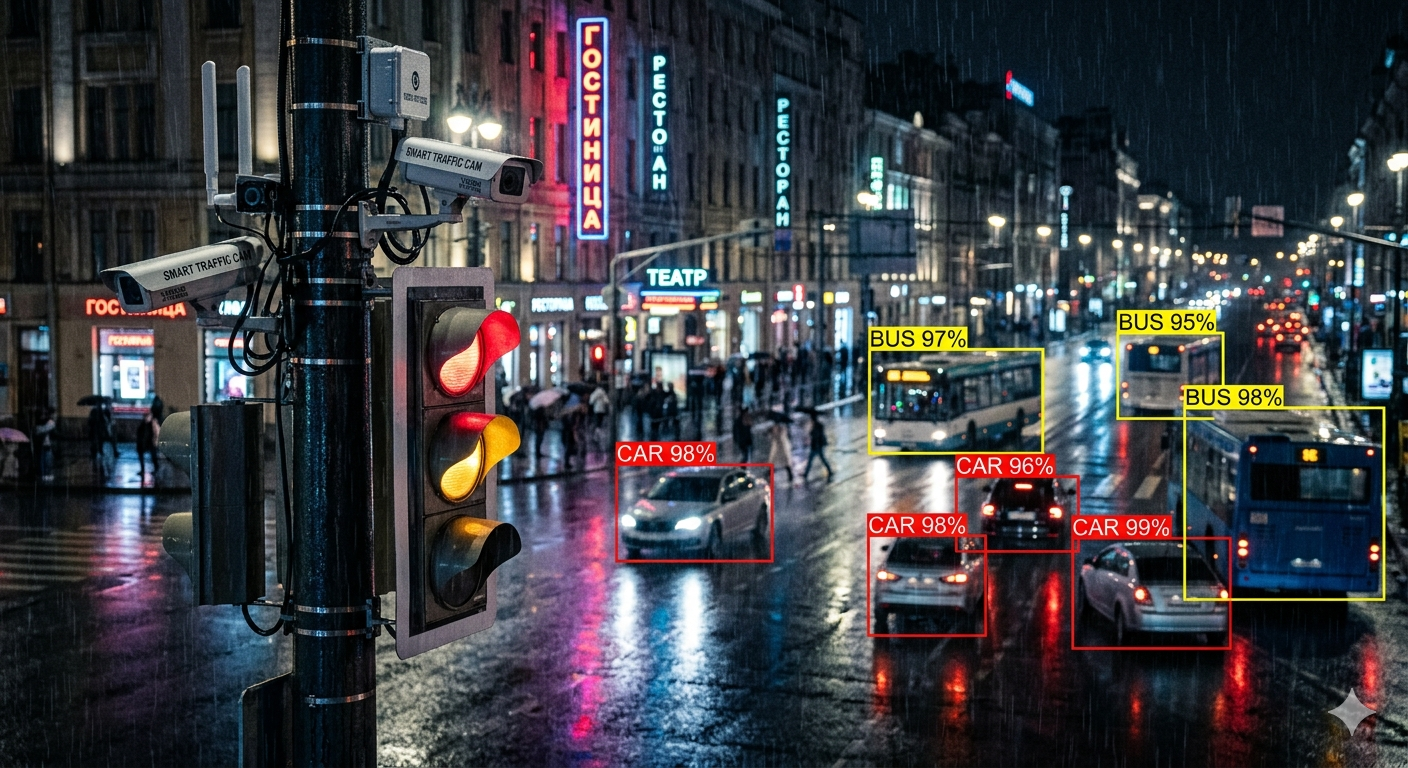
\includegraphics[width=17cm]{z1/3b.png}
	\caption{Итерация 3, модель (b)}
\end{figure}
Изображение хорошо соответствует заданию, за исключением некоторых <<логических>> ошибок.
\subsection{Сравнение моделей}
\begin{table}[h!]
	\centering
	\begin{tabular}{|l|p{5cm}|p{5cm}|}
		\hline
		\textbf{Критерий} & \textbf{модель (a)} & \textbf{модель (b)} \\
		\hline
		Соответствие промпту & 4 & 5 \\
		\hline
		Отсутствие артефактов & 3 & 5 \\
		\hline
		\textbf{Итог} & 3.5 & 5\\
		\hline
	\end{tabular}
\end{table}
Модель (b) справилась лучше чем модель (a), так как генерирует детальное изображение, а также самостоятельно локализует окружение под язык запроса. В свою очередь модель (a) генерирует мыльное/размытое изображение, иногда с нарушенной перспективой.
\subsection{Финальный промпт}
Крупный план умного светофора с встроенными камерами наблюдения и объективами \{ОКРУЖЕНИЕ\}. 
Вокруг каждого автомобиля нарисованы красные рамки выделения (bounding boxes)
как в системах компьютерного зрения с текстом <<CAR \%>>, вокруг каждого автобуса жёлтые рамки с текстом <<BUS \%>> ,
вокруг людей и других объектов нет рамок. \{СТИЛЬ\}
\subsection{Вывод}
В ходе итеративной работы удалось добиться полного соответствия техническому заданию.
Ключевым приёмом стало детальное описание всех элементов сцены и использование стилистических модификаторов
(кинематографичность, глубокая резкость, боке). Даже при отсутствии прямого доступа к параметрам Seed и CFG Scale,
точное формулирование промпта позволило управлять качеством и содержанием изображения. Сравнение моделей показало,
что модель (b) лучше подходит для задач, требующих высокой точности визуализации технических деталей.